\graphicspath{{Chapters/Chapter_ebm/}}


\chapter{Reconstructing missing diagnostics using energy-based models}
\label{ch:ebm}

%\begin{abstract}
 Energy-based models (EBMs) provide a powerful and flexible way of learning relationships in data by constructing an energy surface. We extend EBMs to laboratory plasma physics, a domain characterized by highly nonlinear phenomena studied using incomplete diagnostic information. These diagnostics can be unreliable or difficult to analyze. In addition, the possible configuration space of a plasma device is sufficiently large that it cannot be efficiently searched using conventional analysis techniques. EBMs provide a way to address these issues. At the Large Plasma Device (LAPD), a CNN- and attention-based EBM is trained over a set of randomly generated machine conditions and the corresponding diagnostic time series. We demonstrate diagnostic reconstruction using this EBM and also show that including additional diagnostics improves reconstruction error and generation quality.
%  This model can also be used to infer trends by conditionally sampling along a grid.
  Symmetries in the data can be found by directly evaluating the energy surface, potentially leading to a new line of inquiry using learned models. In addition, this multimodal EBM is able to unconditionally reproduce all distributional modes, suggesting future potential in anomaly detection on the LAPD. Fundamentally, this work demonstrates the flexibility and efficacy of EBM-based generative modeling of laboratory plasma data, and demonstrates practical use of EBMs in the physical sciences.
%\end{abstract}


%TL;DR: Using data from a laboratory plasma device, we demonstrate reconstructing signals, trend inference, and multimodal distribution modeling using a single energy-based model.

\section{Goals and prior work}

\subsection{Goals}
%Nuclear fusion is an upcoming potential energy source that could offset carbon emissions and provide cleaner energy. Developing a fusion reactor is challenging: the environment is hostile to measurement (diagnostics can malfunction or break) and the physics of plasmas is highly nonlinear and dynamical. 
We seek to use machine learning -- particularly generative models -- to alleviate some of the challenges facing fusion-related plasma science and to accelerate the advent of fusion power. In particular, we want to be able to reconstruct missing diagnostic signals from any other set of signals. In addition, the reconstruction should be a probability distribution, not just a single estimate. This distribution should also have the ability to be combined with other sources of information, such as simulations, or constraints placed on it via prior knowledge. 

\subsection{Generative modeling of plasmas}

The use of generative models in plasma physics is not without precedent, but remains relatively uncommon. Variational autoencoders \cite{kingma_auto-encoding_2022} have been used to generate new, realistic output from stellarator transport simulations for inferring trends and uncovering physics \cite{lennart_van_rijn_minimizing_2022} and to discover relationships between inputs and outputs \cite{vos_discovery_2024}. These VAEs have also been used in the COMPASS to identify a rare instability characterized by fluctuations in magnetic probes \cite{skvara_detection_2020} by pertaining on unlabeled data and combining the model with a classifier over a smaller, labeled dataset. 

On the Joint European Torus experiment, a generative topographic map was used to create a 2d representation of a 7d input space (information from 1d profiles) \cite{pau_machine_2019}. This mapping clearly shows a disruptive-nondisruptive boundary and the relative stability of locations in this 2d representation can be evaluated by visualizing cluster distances. Discharge trajectories can be visualized in this reduced 2d space. Likewise on the HBT-EP tokamak, a VAE was trained on coil currents, equilibrium properties, and MHD information to learn a 2d latent representation \cite{wei_dimensionality_2021}. This model was run in real time to identify threshold crossing events which then triggered preprogrammed countermeasures. 

Generative-adversarial networks (GANs) \cite{goodfellow_generative_2014} have also been used to generate synthetic training data (time series of plasma current) for use in training a disruption predictor \cite{dave_synthetic_2023}. GANs have also be used to generate posterior distributions of surface temperature and emissivity given the measured radiance for the thermal surface-pointed cameras on the WEST tokamak \cite{juven_generative_2024}. 

Diagnostic reconstruction is useful in the event a diagnostic goes offline, but it can also be used to supplement existing diagnostics.  One such example is the upsampling of the Thomson scattering signal on DIII-D based on information from other diagnostics using a neural network-based solution \cite{jalalvand_multimodal_2024}. In addition, Bayesian and ML work in fusion has been recently reviewed\cite{pavone_machine_2023}.

Outside of magnetized plasmas, random experiments were performed in an inductively coupled plasma (ICP) similar to the process used to collect for this work. These data were used to train a VAE as a surrogate collisional radiative model \cite{daly_data-driven_2023} to construct an interpolatable latent representation.

Concerning EBMs, they have yet to be applied to plasma physics problems. One notable application in the physical sciences has been in the high-energy physics community. EBMs were used for modeling event patterns in the Large Hadron Collider (LHC) for anomaly detection and to augment a classifier \cite{cheng_versatile_2024} with success.

%They trained two models: one where the inputs were known, and another where they were unknown (from ray-traced simulations). The GAN accurately captured the posterior distribution (and uncertainties) for both cases.

%Really cool paper using VAEs to create a surrogate collisional radiative model in an ICP device \cite{daly_data-driven_2023}. A good portion of this work was finding the appropriate latent dimension size to get good, interpolatable latent representation. This latent space was scanned and compared with some experimental results, which looks promising. This is the only other work I've found where data were collected in a random / diverse fashion. 

%VAEs were used with partially-labeled data from the COMPASS tokamak to identify chirped Alfv\`en eigenmodes \cite{skvara_detection_2020}. They approached the identification problem in two ways: treating it as an out-of-distribution identification problem, and as a partially-supervised learning problem by pretraining a VAE and then combining that with a classifier on a smaller, labeled dataset (the latter of which was superior). The pretrained latent space was used for determining the class of the labeled data.  

\section{Introduction to energy-based models (EBMs)}

Energy-based models interpret a probability distribution through the lens of the Boltzmann distribution \cite{hopfield_neural_1982, ackley_learning_1985, lecun_tutorial_2006}. In the EBM formulation, the unnormalized probability density is parameterized by an energy function, that is $\tilde{p}(\bf{x}) = \exp(-E_\theta(\bf{x}))$, where $\theta$ are the parameters of this energy function. In this work and the works cited, this energy function is parameterized by a neural network. EBMs have been historically difficult to train, but recent work has demonstrated high-quality sampling using MCMC techniques in high-dimensional spaces \cite{du_model_2019, du_implicit_2020, du_improved_2021, du_compositional_2020, du_unsupervised_2021, nijkamp_anatomy_2020, nijkamp_learning_2019, deng_residual_2020, gao_learning_2018}. These MCMC techniques are fundamentally based in contrastive divergence \cite{hinton_training_2002, ruslan_deep_2009, tieleman_training_2008}. The nature of MCMC-based sampling of EBMs, detailing the convergence and expansion and contraction of learned models (a paradigm particularly helpful for training EBMs in this work) has been studied \cite{nijkamp_anatomy_2020, nijkamp_learning_2019}. Training via contrastive divergence can be improved by implementing a term typically left out which approximates the KL-divergence \cite{du_improved_2021}. 

EBMs can attain GAN-like performance while generating all modes of a distribution \cite{du_implicit_2020}. These models have also been used for text generation \cite{deng_residual_2020} and model-based planning \cite{du_model_2019}. In addition, EBMs can be composed by combining the energy functions in various ways which has been demonstrated in image generation tasks \cite{du_compositional_2020, du_unsupervised_2021}.

Overview of EBMs, how they are trained, and their place among generative models \cite{carbone_hitchhikers_2024}. Another helpful review of generative modeling that helped in the selection by detailing advantages and disadvantages of various methods \cite{bond-taylor_deep_2021}. EBMs in particular have some desirable properties. The implicit generation scheme does not require balancing an explicit generator with a discriminator or encoder. In addition, the energy-based representation is amenable to modification of an auxiliary function, allowing the generated samples to be easily steered, enabling the composition of multiple energy functions. Lastly, EBMs do not easily suffer from mode collapse or otherwise ignore parts of the distribution. For these reason we use EBMs for building a distribution of our LAPD data.

%VAE paper \cite{kingma_auto-encoding_2022}
%GAN paper \cite{goodfellow_generative_2014}
%One of the earlier MCMC-based EBM papers \cite{gao_learning_2018}.
%.Hopfield nets:. Deep Boltzman Machines used contrastive divergence \cite{ruslan_deep_2009}. Persistent contrastive divergence: \cite{tieleman_training_2008}.


\section{Data preparation}

Around 130 thousand shots were taken on the Large Plasma Device for 67 different dataruns, varying machine conditions and probe configurations as detailed in chapter \ref{ch:ml-dataruns}. The train-test split identical to what was performed in earlier chapters. Namely, four dataruns each from \texttt{DR1} and \texttt{DR2} were held out as representative configurations. In order to reduce computational requirements, the time series data was downsampled. The original sampling rates for the machine state information and auxiliary diagnostics was 25 kHz. The sampling rate for the $I_\text{sat}$ probe was 6.25 MHz. All time-series data were downsampled to a common sampling rate of 2.5 kHz. This downsample leads to the time series having a length of 76 points long, and the MSI were truncated to be identical in duration and start time to the $I_\text{sat}$ time series.

The dataset includes nine time series in total: discharge current, discharge voltage, 5 diode signals (the last of which having a He-II filter), interferometer (line-integrated density), and $I_\text{sat}$ from a Langmuir probe. Additionally, several one-dimensional inputs and flags were included: probe position (x, y, z), magnetic field (source, mirror, and midplane), gas puff duration and voltage, total gas pressure, first 4 amu RGA readings, run set flag, and top gas puff flag. In total, the input length is 699 features when concatenated. 

When fed into the model, each input is mean-subtracted and scaled independently by the peak-to-peak value. Scaling each value was found to work much better than scaling a whole time series by the same value. Often, the beginning and end of the time series would have very little variance (such as in discharge current always starting at 1 kA). Learning distributions of very small width  appears to be difficult for EBMs. 

%An additional dataset of 29 million shots was collected over the span of 3 years

\section{Training the EBM}
The following loss function is used to train the EBM:
\begin{equation}
	\mathcal{L} = \mathcal{L}_\text{CD} + \mathcal{L}_\text{KL} + \alpha \mathcal{L}_\text{reg}
\end{equation}
where $\mathcal{L}_\text{CD}$ is the contrastive divergence loss, $\mathcal{L}_\text{KL}$ is the KL-divergence loss, and $\mathcal{L}_\text{reg}$ is the energy regularization loss, listed in order of importance.
The contrastive divergence loss is defined as:
\begin{equation}
	\mathcal{L}_\text{CD} = \frac{1}{M} \sum_i E_\theta(\tilde{x}_{i}^+) - E_\theta(\tilde{x}_{i}^L)
\end{equation}
This loss calculates the difference in energies between sample from the energy surface $\tilde{x}_{i}^L$ via Langevin dynamics -- the ``negative'' samples -- and the samples from the data distribution $\tilde{x}_{i}^+$, i.e., the training data. This loss places the energy surface in tension, with the surface being pulled down by the data and pushed up on the negative samples. Both terms must be included: absence of negative samples would lead to a vacuous solution such as a flat energy surface.
The KL-divergence loss is:
\begin{equation}
	\mathcal{L}_\text{KL} = \frac{1}{M} \sum_i E_{\Omega(\theta)}(E_\theta(\hat{x}_{i}^K) - \text{NN}(X, \hat{x}_{i}^K)
\end{equation}
This loss, suggested in \cite{du_improved_2021} includes portions of the CD typically left out. Namely, this loss minimizes the sampler energy by propagating gradients through the MCMC steps themselves instead of the final samples. In addition, the nearest-neighbor (\texttt{NN}) samples are used to estimate the energy of the negative samples so that the entropy of the distribution is maximized. This loss, though not necessary, significantly improves training stability. 
The regularization loss
\begin{equation}
	\mathcal{L}_\text{reg} = \frac{1}{M} \sum_i E_\theta(\tilde{x}_{i}^+)^2 + E_\theta(\tilde{x}_{i}^L)^2
\end{equation}
keeps the energy values centered near 0. The absolute value of the energy does not matter -- only the gradients and scale -- but this  is included to keep the results easily interpretable and to avoid extreme energy values as to not run into floating-point representation boundaries. In this work, the scale of this regularization is very small with $\alpha = 1 \times 10^{-6}$. This loss also functions as a great diagnostic for when the sampler fails: the regularization loss will reach $1/\alpha$. The EBM training process is broken down in algorithm \ref{alg:training}.

\begin{algorithm}
\caption{EBM training algorithm}\label{alg:training}
%\small
\begin{algorithmic}
\Require Training samples $x_i^+$, training data distribution $\mathcal{}p_D$, energy function $E_\theta$, replay buffer $\mathcal{B}$, step size $\epsilon$, MCMC steps $L$, KL MCMC steps $K$, energy regularization strength $\alpha$, stop gradient operator $\Omega(\cdot)$, replay fraction $f_\mathcal{B}$, batch size $M$

	\State $\mathcal{B} \gets \mathcal{U}(-1,1)$ \Comment{Fill buffer from uniform distribution}

	\While{not converged}
		\State $x_i^+ \sim \mathcal{}p_D$
		\State $\tilde{x}_{i}^0 \sim \mathcal{B}$ sample $M f_\mathcal{B}$ negative examples, $\mathcal{U}(-1,1)$ otherwise
		\State $X \sim \mathcal{B}$ nearest-neighbor samples such that $X \cap \tilde{x}_{i}^0 = \varnothing$
		\\
		\For{sample step $\ell=1$ to L}  \Comment{Run Langevin dynamics}
			\State $\tilde{x}_{i}^\ell \gets \tilde{x}_{i}^{\ell-1} - \frac{\epsilon^2}{2}\nabla_x E_\theta(\tilde{x}_{i}^{\ell-1}) + \epsilon \mathcal{N}(0, 1)$
		\EndFor
		\State $\tilde{x}_{i}^{L} = \Omega(\tilde{x}_{i}^{L})$
		\\	
		\State $\hat{x}_{i}^0 = \tilde{x}_{i}^\ell$ where $\ell = L-K$ \Comment{Run Langevin dynamics for KL loss}
		\For{KL sample step $k=1$ to K}
			\State $\hat{x}_{i}^k \gets \hat{x}_{i}^{k-1} - \frac{\epsilon^2}{2}\nabla_x E_\theta(\hat{x}_{i}^{k-1}) + \epsilon \mathcal{N}(0, 1)$ 
		\EndFor
		\\
		\State $\mathcal{L}_\text{CD} = \frac{1}{M} \sum_i E_\theta(\tilde{x}_{i}^+) - E_\theta(\tilde{x}_{i}^L)$ 
		\State $\mathcal{L}_\text{KL} = \frac{1}{M} \sum_i E_{\Omega(\theta)}(E_\theta(\hat{x}_{i}^K) - \text{NN}(X, \hat{x}_{i}^K)$ \Comment{Has gradients through MCMC}
		\State $\mathcal{L}_\text{reg} = \frac{1}{M} \sum_i E_\theta(\tilde{x}_{i}^+)^2 + E_\theta(\tilde{x}_{i}^L)^2$
		
		\State $\mathcal{L} = \mathcal{L}_\text{CD} + \mathcal{L}_\text{KL} + \alpha \mathcal{L}_\text{reg}$
		\\		
		\State Apply $\nabla_\theta \mathcal{L}$ to $\theta$ via the Adam optimizer

		\State $\mathcal{B} \gets \mathcal{B} \cup \mathcal{U}(-1,1)$ and remove samples to maintain buffer size
	\EndWhile
	
\end{algorithmic}
\end{algorithm}

\subsection{The sampler}

The sampler is fundamental to how the model is trained and how samples are generated; the configuration of the sampler is one of the most important considerations when building the EBM. The samples are initialized from random noise between $-1$ and 1. We use Langevin dynamics to move the samples as formulated in Nijkamp et al. \cite{nijkamp_anatomy_2020}, as seen in algorithm \ref{alg:sampling}. A variety of step sizes and number of steps were used. The number of sampler steps per batch was critical for training stability: 30 appears to be close to the minimum number of steps for stable training, similar to what has been observed in other studies \cite{cheng_versatile_2024}.

The step size is typically chosen to match the standard deviation of the smallest feature, but that was found to be too large for this use case. Given that our data is highly multimodal, some modes of the input distribution had a deviation of 0 (such as the flags).  For this reason, a smaller step size of $\epsilon = 0.01$ was used. 

\begin{algorithm}
\caption{EBM sampling}\label{alg:sampling}
%\small
\begin{algorithmic}
\Require Energy function $E_\theta$, auxiliary energy function $F$, step size $\epsilon$, MCMC sampling steps $L$
	\State $\tilde{x}_{i}^0 \sim \mathcal{U}(-1,1)$ \Comment{Initialize on uniform distribution}
	\For{sample step $\ell=1$ to L}  \Comment{Run Langevin dynamics}
		\State $\tilde{x}_{i}^\ell \gets \tilde{x}_{i}^{\ell-1} - \frac{\epsilon^2}{2}\nabla_x \left( E_\theta(\tilde{x}_{i}^{\ell-1}) + F(\tilde{x}_{i}^{\ell-1}) \right)+ \epsilon \mathcal{N}(0, 1)$
	\EndFor
	\\
	\State Return $\tilde{x}_{i}^{L}$
	
\end{algorithmic}
\end{algorithm}

The model was trained for 27 hours over 172 epochs. The  The batch size was 128 and was trained with the AdamW optimizer with a learning rate of $10^{-4}$, decaying to $10^{-5}$ after 20 epochs. Training using stochastic gradient descent required very large learning rates ($10^{-2}$) and could not generate realistic samples even with a learning rate decay schedule. The first 100 epochs were trained in a single run; the next 72  were resumed from the final checkpoint of the previous run, leading to reinitialization of the replay buffer. Given the low learning rate, this did not have a significant impact on model training. The model used for inference was from the 39th epoch into this second run, after which training diverged. 

The training curves of loss, relative energy, and energy gradient can be seen in fig. \ref{fig:losses-energies}. The loss curve is very hard to interpret given all the components of the loss function. Maintaining a relative energy near 0 between negative and positive samples is crucial for model performance. A value near 0 indicates that the generated samples are close to the data distribution. When the sampler diverges, samples are no longer accurately representing the data and thus training fails. The energy function learns the scale of the gradients required to produce good samples. When training is proceeding normally, the ratio of the gradient step to the noise scale (step size) $\epsilon$ is near 1. 

\begin{figure}
	\centering
	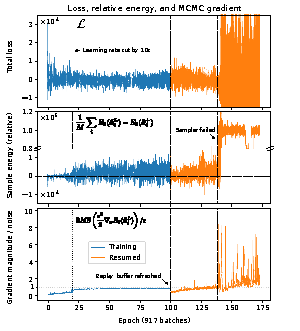
\includegraphics[width=\linewidth]{figures/losses-energies-rasterized.pdf}
	\caption{\label{fig:losses-energies}Training curves of the model. Top: the total loss, middle: the relative energies of the negative samples and the training examples (positive samples), bottom: the gradient of the energy function normalized to the noise scale (step size $\epsilon$). \todo{replace with non-rasterized version}}
\end{figure}

\subsection{Replay buffer configuration}
A replay buffer is used to provide a warm start for the sampler chains. Every batch iteration, 5\% of the samples from the buffer are replaced with random noise (a replay fraction of 0.95). This replay fraction leads to a mean of 1/0.05=20 batch iterations for each chain, with half the chains experiencing $\ln(2)/0.05 \approx 14$ batches. The replay buffer requires 4 to 5 epochs to converge to an exponential distribution in the number of steps experienced by each chain in the buffer. This diversity of chain lengths likely encourages quick convergence of the chain but good long-term samples (on average, each chain experience 600 MCMC updates/steps). The distribution of the batches among the replay buffer can be seen in fig. \ref{fig:buffer_distribution}. One downside of this long buffer is that if a sample ends up in a region far outside the domain ($-1$ to 1) it can cause exploding gradients; samples have a $\approx$ 50\% chance of lasting 194 batches if one goes awry. Implementing a reject step for this prodigal samples may improve training stability. 

\begin{figure}
	\centering
	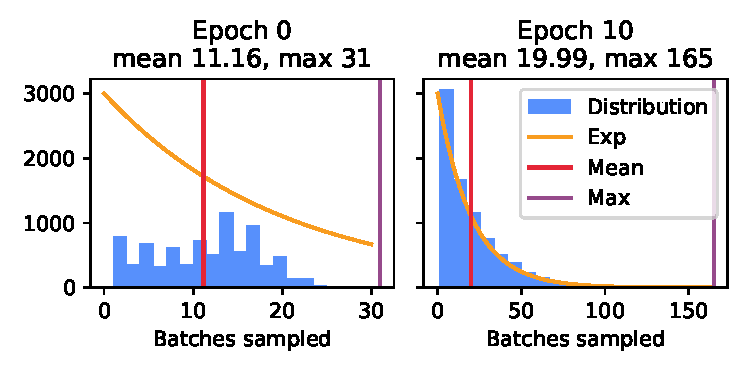
\includegraphics[width=350pt]{figures/buffer_distributions.pdf}
	\caption[Distribution of batches in replay buffer samples]{\label{fig:buffer_distribution}Distribution of batches in replay buffer. When training is starting (epoch 0, left), the number of batches each sample experiences is low and somewhat uniform. After 10 training epochs (right), the number of batches experienced by a sample converged to an exponential distribution.}
\end{figure}

\subsection{Sampling behavior}
In general, if the model is not learning, increase the number of sample steps, decreasing the step size, and decreasing the learning rate are beneficial steps to take. A lower learning rate decreases the change per batch in the energy surface, so stale sample chains from the replay buffer may find themselves in more familiar territory than if the energy function is rapidly changing. More sample steps relaxes the requirement for the samples to rapidly find realistic (lower energy) locations, perhaps leading to shallower gradients and greater stability. Much work needs to be done to really understand the dynamics of the sampler in the training process. The samples from the replay buffer sampling may also benefit from a non-memoryless distribution so that the chains are guaranteed a certain number of sample steps over their lifetime, with a hard limit so that chains do not persist for too long. 

\section{Architecture}

The model is intrinsically multi-modal: time-series data from diagnostics is mixed in with machine settings, state, and probe position. In this model we preprocess separately each time series and the LAPD configuration. Convolutional NNs were used for the time series input, and transformer-like multi-head attention blocks were used for the settings, state, and probe position. The time series convolutions were merged in another convolutional pass, and the two branches were combined using multi-head attention.  A visual representation of the architecture can be seen in fig. \ref{fig:architecture}, with the layer blocks defined in fig. \ref{fig:architecture_blocks}. Convolutions were chosen for the time series input because they are relatively parameter efficient.  The depth of the network guarantees that the receptive field of the downstream neurons covers the entire input space so the positional dependence of the signal is maintained. No pooling layers were used. In general, fully-connected networks were found to be difficult to train (which has been observed in other studies \cite{cheng_versatile_2024}) and are only used when projecting representations to higher or lower dimensions. The cause of this training difficulty for dense networks is unknown. In general, including residual connections appeared to help training stability.

\begin{figure}
	\centering
	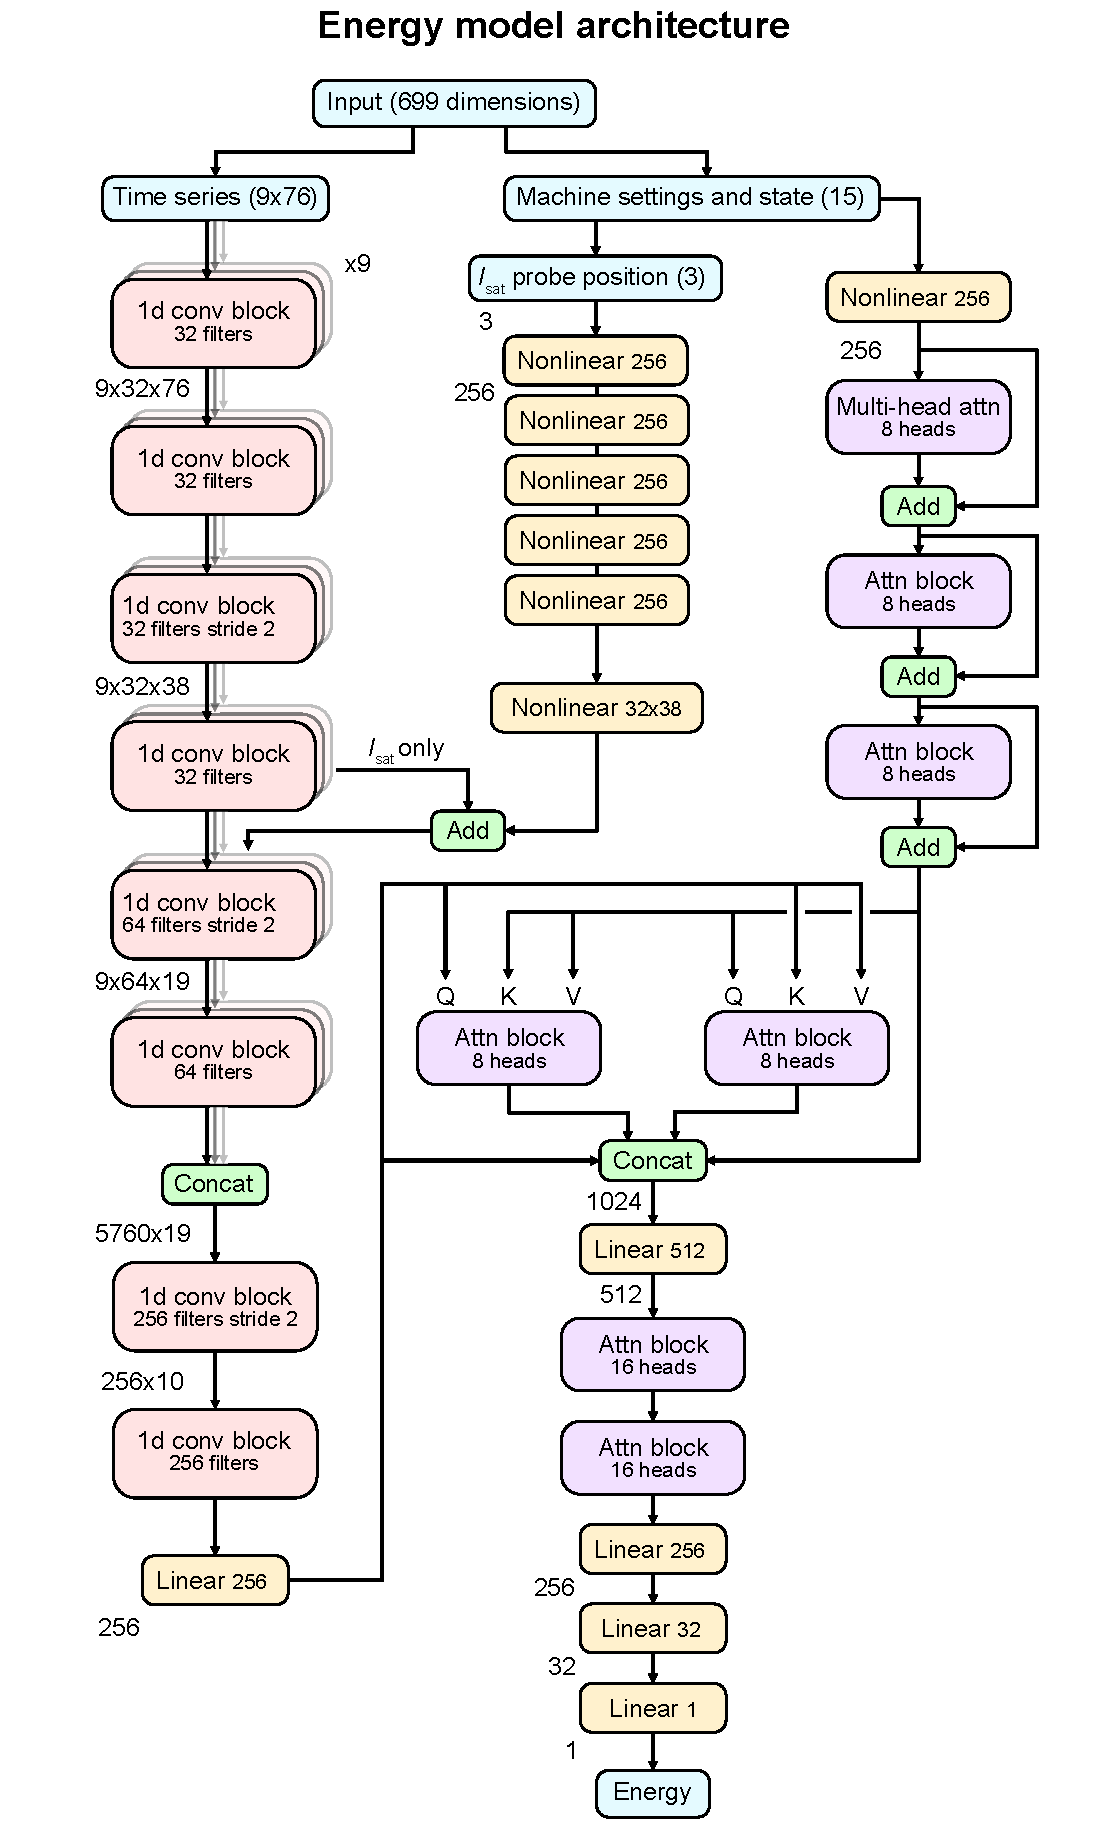
\includegraphics[height=550pt]{figures/architecture.pdf}
	\caption{\label{fig:architecture}Architecture for learning the energy function. Two main branches were used: processing the time series inputs and the machine settings. The layer blocks are defined in fig. \ref{fig:architecture_blocks}.}
\end{figure}

\begin{figure}
	\centering
	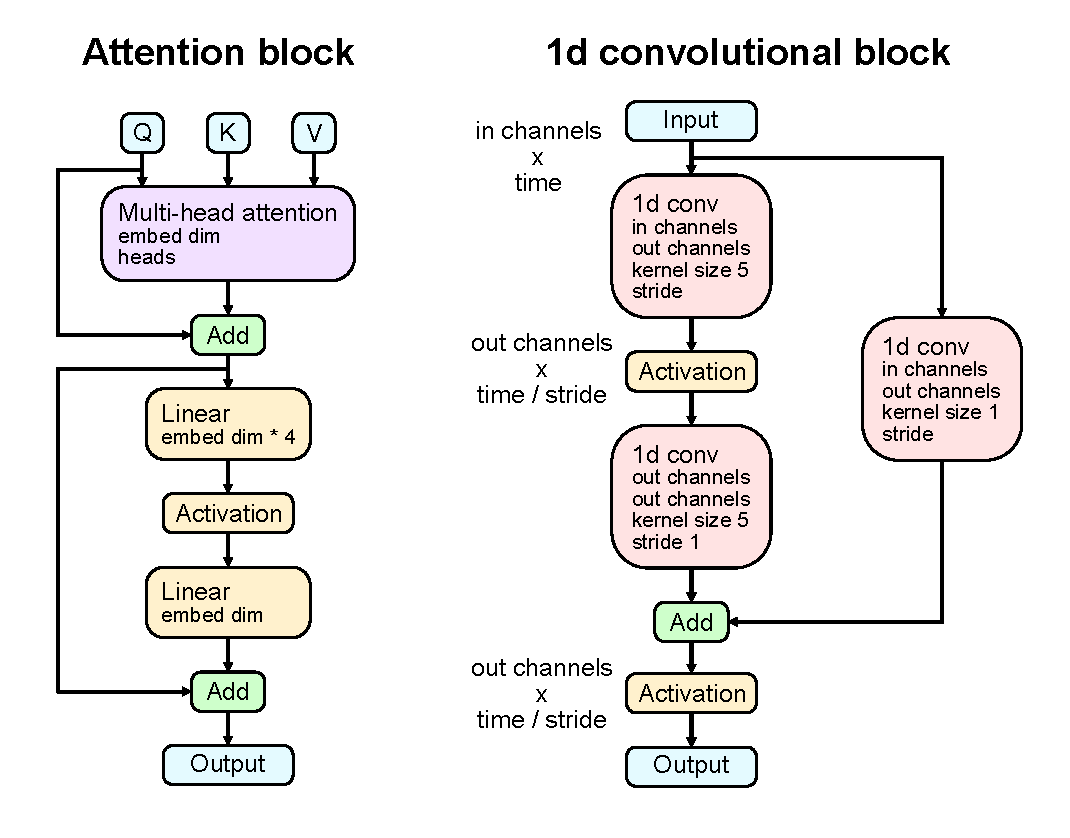
\includegraphics[width=\linewidth]{figures/architecture_blocks.pdf}
	\caption{\label{fig:architecture_blocks}Layer blocks used in the EBM architecture. Residual layers work well.}
\end{figure}

During experimentation, it was found that preprocessing the signals before combining into the energy function worked much better than combining all the signals near the inputs. This may indicates that feature learning is very important for the EBM to learn a representative energy surface, at least for this dataset. The energy layers -- responsible for combining the learned representations -- were not as sensitive to parameter count. Despite this importance of feature learning, attempts to train the EBM with a pretrained encoder was difficult and could not converge to a good energy surface.

The EBM struggled to model the positional dependence of the $I_\text{sat}$ signal, so a branch was added from the probe positions to add onto the intermediate representation of the $I_\text{sat}$ signal. This branch improved performance of the positional mapping, but is not as accurate as the simple feed forward model from the previous chapter. Performance may be improved by improving model capacity, or reducing the learning rate in conjunction with the step size. 

The architecture developed for this study is not optimal -- it is simply one that works and is mostly stable. The architecture likely has ample room for improvement, particularly regarding the learning of the probe position. Additional, intermediate connections between the time series and 1d inputs should be explored. The current architecture can be thought of as a medium-term multimodal fusion design (early fusion did not work). 


\section{Unconditional sampling}

Unconditional samples can tell us how well the network is modeling the data distribution. 5000 samples were generated with the inputs initialized from a uniform distribution between -1 and 1. These samples ran for 120 steps of Langevin dynamics with the default step size of 0.01. On an RTX 3090, this process took 64 seconds. The MCMC trajectories of unconditional samples steps these samples can be seen in fig. \ref{fig:uncond_mcmc}. Notably after a small number of sampling steps -- around 30 -- the energy surface gradients appear to flatten out and thus the energies of the samples level off. This leveling point may be determined by the number of samples steps used while training the model: each randomly-initialized sample runs for 30 steps before being added to the replay buffer. Despite converging relatively quickly, long-run MCMC chains look just as realistic as shorter-duration chains and do not exhibit the burn-in or high-saturation that has been observed in other work \cite{du_implicit_2020}. 

\begin{figure}
	\centering
	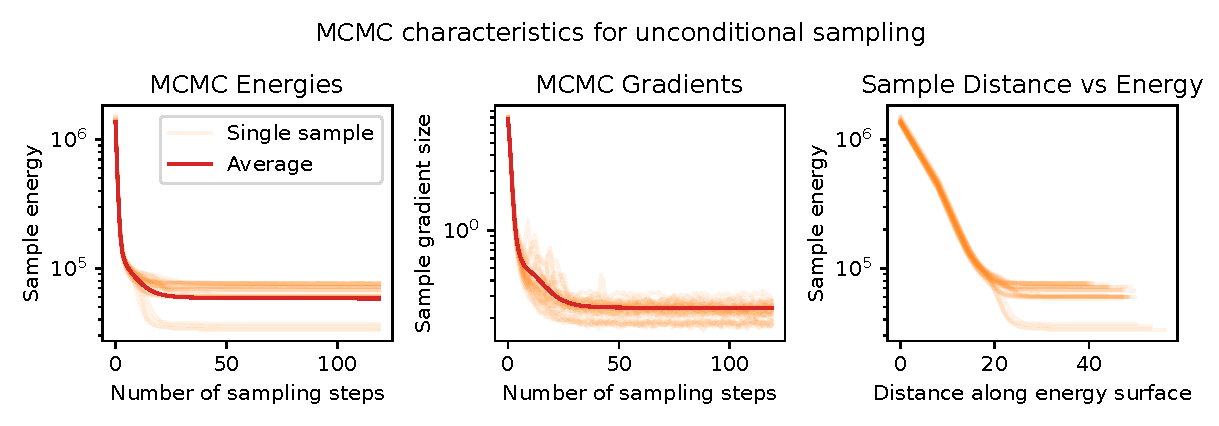
\includegraphics[width=\linewidth]{figures/uncond_mcmc_diagnostics_39-0.pdf}
	\caption[MCMC energies, gradients, and integrated trajectory length for unconditional samples]{\label{fig:uncond_mcmc}MCMC energies, gradients, and integrated trajectory length for unconditional samples. Left: the model converges after approximately 50 sampling steps. Middle: the gradients approach an asymptote; long-term samples are realistic. Right: integrated trajectory length show that individual MCMC trajectories vary in total distance traveled along the energy surface.}
\end{figure}

Given that the data distributions are highly multi-modal, it is important that the EBM captures many, if not all, modes of the distribution. Representative examples of these distributions, namely of diode 3 at 16 ms (chosen arbitrarily) and the mirror field, can be seen in fig. \ref{fig:uncond_examples}. The full unconditional distribution for each input (or at 16 ms for time-series data) can be seen in fig. \ref{fig:uncond_dist_full}. Notably, although most -- if not all -- modes of the distribution are covered, the mass associated with each mode may not agree. This behavior is evident in the aggregate energy distribution seen in fig. \ref{fig:uncond_energy}. On average, the unconditional samples have higher energy than the data. In terms of the scaled values of all of the inputs, the model appears to struggle to model extreme values. This could hint towards the need for data augmentation so that chains can properly mix, or a need for a different random initialization before commencing Langevin dynamics.

\begin{figure}
	\centering
	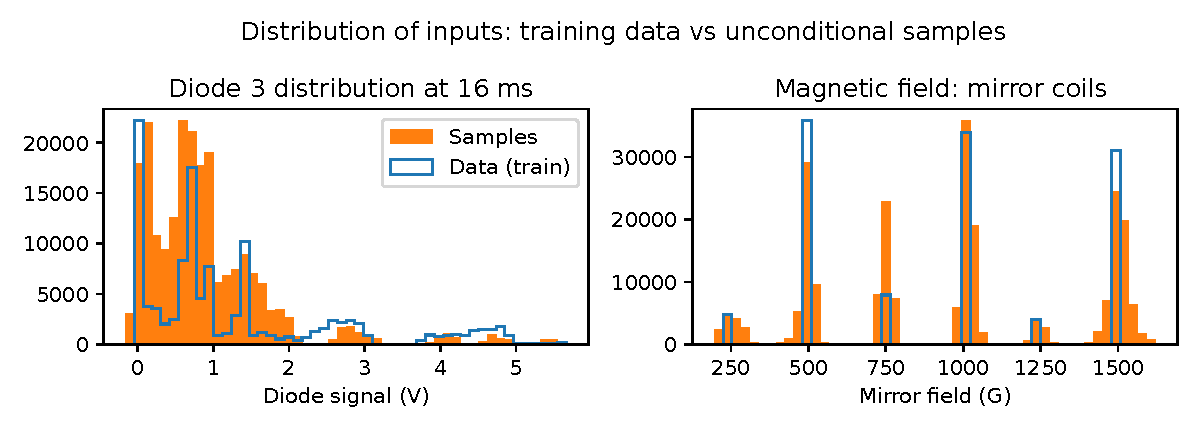
\includegraphics[width=\linewidth]{figures/uncond_diode-3_B-mirror_39-0.pdf}
	\caption[Unconditional samples -- diode 3 and mirror field]{\label{fig:uncond_examples}Unconditional samples of diode 3 at 16 ms and the mirror coil magnetic field inputs, chosen as representative examples. The EBM learns all modes of the distributions, though the probability mass is not well-aligned.}
\end{figure}

\begin{figure}
	\centering
	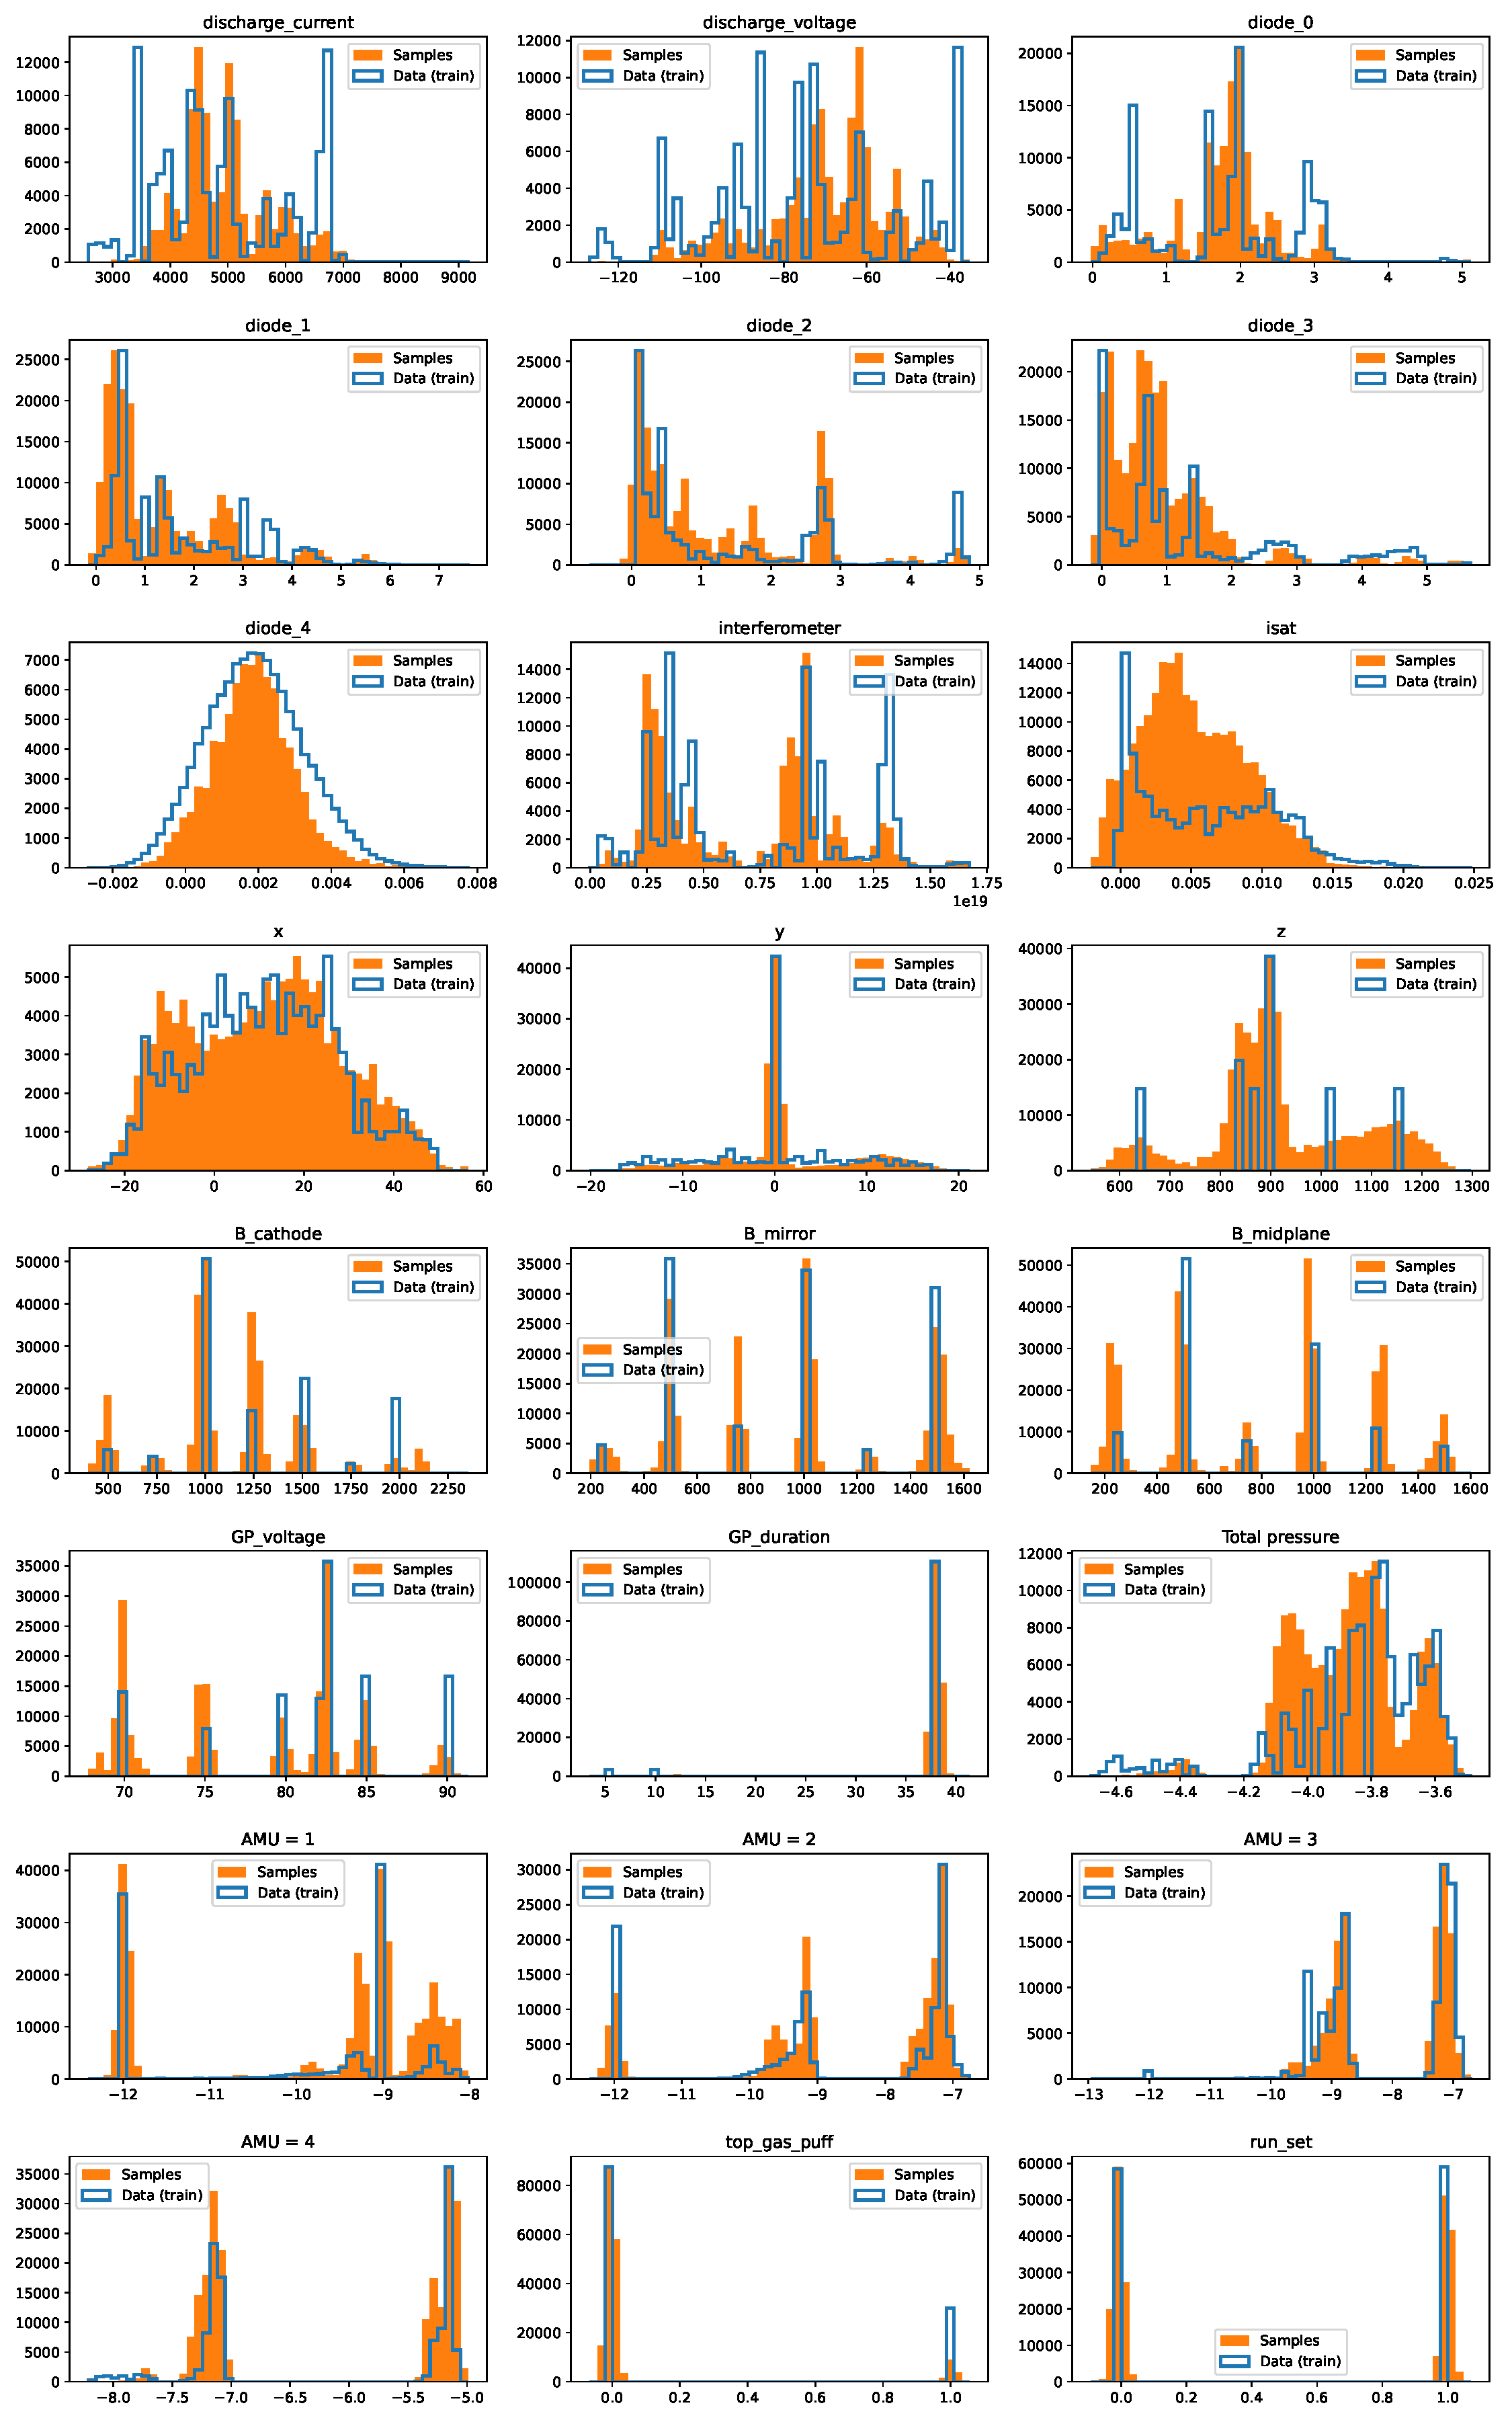
\includegraphics[width=300pt]{figures/uncond_histograms_39-0.pdf}
	\caption[Unconditional samples -- all inputs]{\label{fig:uncond_dist_full}Unconditional samples of all inputs, or at 16 ms -- chosen arbitrarily -- for time series. The model appears to learn most, if not all, modes of the distributions, but can perform poorly when modeling the probability mass, such as in the $I_\text{sat}$ distribution.}
\end{figure}

\begin{figure}
	\centering
	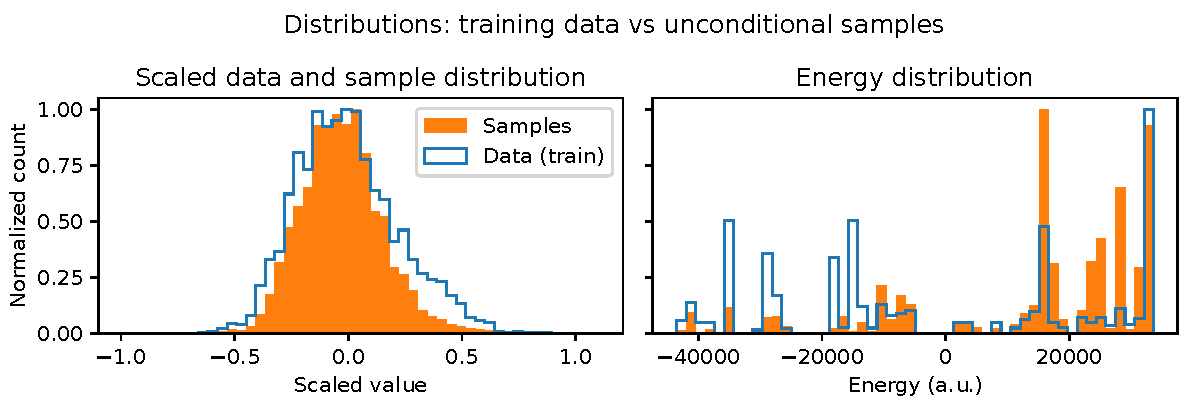
\includegraphics[width=\linewidth]{figures/uncond_histograms_merged_energy-dist_39-0}
	\caption[Histograms of scaled values and energy for unconditional samples]{\label{fig:uncond_energy}Left: all scaled inputs from the training set vs samples inputs. The distributions are similar, but the EBM does not appear to learn more extreme values. Right: corresponding energy distribution. The EBM learns all the modes, but the probability mass is not properly distributed.}
\end{figure}

Given that the EBM learns the unconditional data distribution well, it should be able to perform well for anomaly detection. When a particular component of the input is outside the expected joint distribution, the energy will be higher and, when compared to usual negative samples, will clearly be an outlier.

\section{Diagnostic reconstruction via conditional sampling}

Conditional sampling of these models is typically performed by initializing portion of the inputs on real (or otherwise desired) data and only sampling the other inputs. In practice, this can be done by freezing the gradients of the inputs to be conditioned on. In this work, we use a different approach of instead modifying the energy function based on the data to be conditioned on. Given the energy model $E(x)$, where $x$ is an input into the model, we add an auxiliary energy function $F(x)$ that is added to $E(x)$. This creates a new aggregate energy function $E(x) + F(x)$. By definition of energy $p_E(x) \propto \exp(-E(x))$, this is equivalent to multiplying the two distributions $p_E(x) \cdot p_F(x)$. In other words, adding this auxiliary energy function $F(x)$ to $E(x)$ implies we are sampling over the distribution $p_F \cap p_F$.

The choice of auxiliary energy function $F(x)$ can make a large difference on the conditional samples. We choose $F(x)$ to be a quadratic energy function centered on the data: 
\begin{equation}
	F(x) = \left(\frac{x - x_\text{fixed}}{\sigma_F} \right)^2
\end{equation}
where $\sigma_F$ controls the horizontal scale of the quadratic function. Interpreted as a probability distribution, this is a Gaussian with standard deviation $\sigma_F$. The minimal width for stable sampling appears to be $\approx (2 \epsilon)^2$. This makes sense from a sampling point of view: if the width of $F(x)$ approach the step size, a Langevin update step may place the particle at a much higher energy with much larger gradients. This behavior also ties the conditional sampling directly to the training process because the conditional samples are naturally limited to the step sized used while training, and thus are also tied to the fidelity of the model. Other distributions were used, such as a Laplace distribution via $F(x) = \vert x - x_\text{fixed} \vert$, but the samples produced lacked the diversity seen when using a quadratic $F(x)$. Note that the normalizing constants of the probability distribution $p_F(x)$ do not matter because they vanish after $-\log(\cdot)$ is applied and the energy gradients $\nabla_x F(x)$ are taken.

\subsection{Sampling interferometer signals}

Using this conditional sampling method, we now reconstruct interferometer signals. We choose to reconstruct interferometer signals because the results are more easily interpreted physically than the diodes and the discharge current. Using conditional sampling, we compare the samples when only the LAPD control inputs are given and compare with sampling when other diagnostics are given, namely the discharge current, diodes, and $I_\text{sat}$. The machine inputs are the discharge voltage, gas puff duration and voltage, gas pressures, and magnetic field configuration. We also compare the traditional method of initializing on data and freezing gradients. A summary of the results and standard deviation of the distributions can be seen in table. \ref{tab:ifo-cond-sample}. The full time series of the samples can be seen in fig. \ref{fig:ifo_sample}. Note that the training set RMSE is an order of magnitude better than the test set, which is in line with expectations given the limited dataset diversity.

\begin{table*}
\small
	\centering
	\caption{RMSE and 2$\sigma$ of conditional interferometer samples for test set and \texttt{DR2\_02}}
	\label{tab:ifo-cond-sample}
	\begin{tabular}{l l l l}
		Given: & LAPD settings only & All signals & Frozen gradients \\
		\hline
		RMSE (test set) & $4.12 \times 10^{18}$ & $2.91 \times 10^{18}$ & $3.13 \times 10^{18}$ \\
		RMSE (\texttt{DR2\_02})& $3.77 \times 10^{18}$ & $3.54 \times 10^{18}$ & $2.51 \times 10^{18}$ \\
		2 $\sigma$ (\texttt{DR2\_02}) & $6.93 \times 10^{18}$ & $8.37 \times 10^{18}$ & $3.38 \times 10^{17}$ \\
		\hline
		Training RMSE & $4.40 \times 10^{17}$ \\
	\end{tabular}
\end{table*}

For sampling, 90 samples steps were taken with the training step size of $\epsilon=0.01$. The auxiliary energy function used a width of $(2\epsilon)^2$. Interferometer traces from a single shot from each of the eight test set dataruns were sampled. 128 samples of the interferometer signal were taken from each datarun, taking approximately 9 seconds on an RTX 3090. 

Sampling with only machine inputs given led to a large variety of potential interferometer signals, seen on the left of fig. \ref{fig:ifo_sample}. Comparing to the case where all data is given (middle of the figure) yields some interesting insights. First , the variety of the sample distribution is dramatically decreased (seen in the bottom row). The number of modes in the distribution dramatically decreased from over ten to four. Second, the shapes of the curves when diagnostics are given matches better. Third, the RMSE improves a little bit for this particular case, but reduces significantly -- $\gtrsim 25$\% -- when computed over the entire test set (tab. \ref{tab:ifo-cond-sample}). The $2 \sigma$ range of the samples increases, however, perhaps indicating increased uncertainty, though that is counterintuitive given the increased context. The particular $I_\text{sat}$ time trace did not make much of a difference on sample quality, indicating that the model was also using information in the discharge current and diode signals when reconstructing the interferometer signal.

Sampling while freezing gradients (right side of fig. \ref{fig:ifo_sample}) can lead to good RMSE values relative to the other samples, but the actual samples look terrible and are unphysical: negative density is impossible. Constraining the samples to be greater than 0 using an auxiliary energy function ensures positive interferometer values, but the sample quality remains very poor and ironically increases the RMSE. The distribution of signals is also very narrow, leading to a very overconfident prediction. 

\begin{figure}
	\centering
	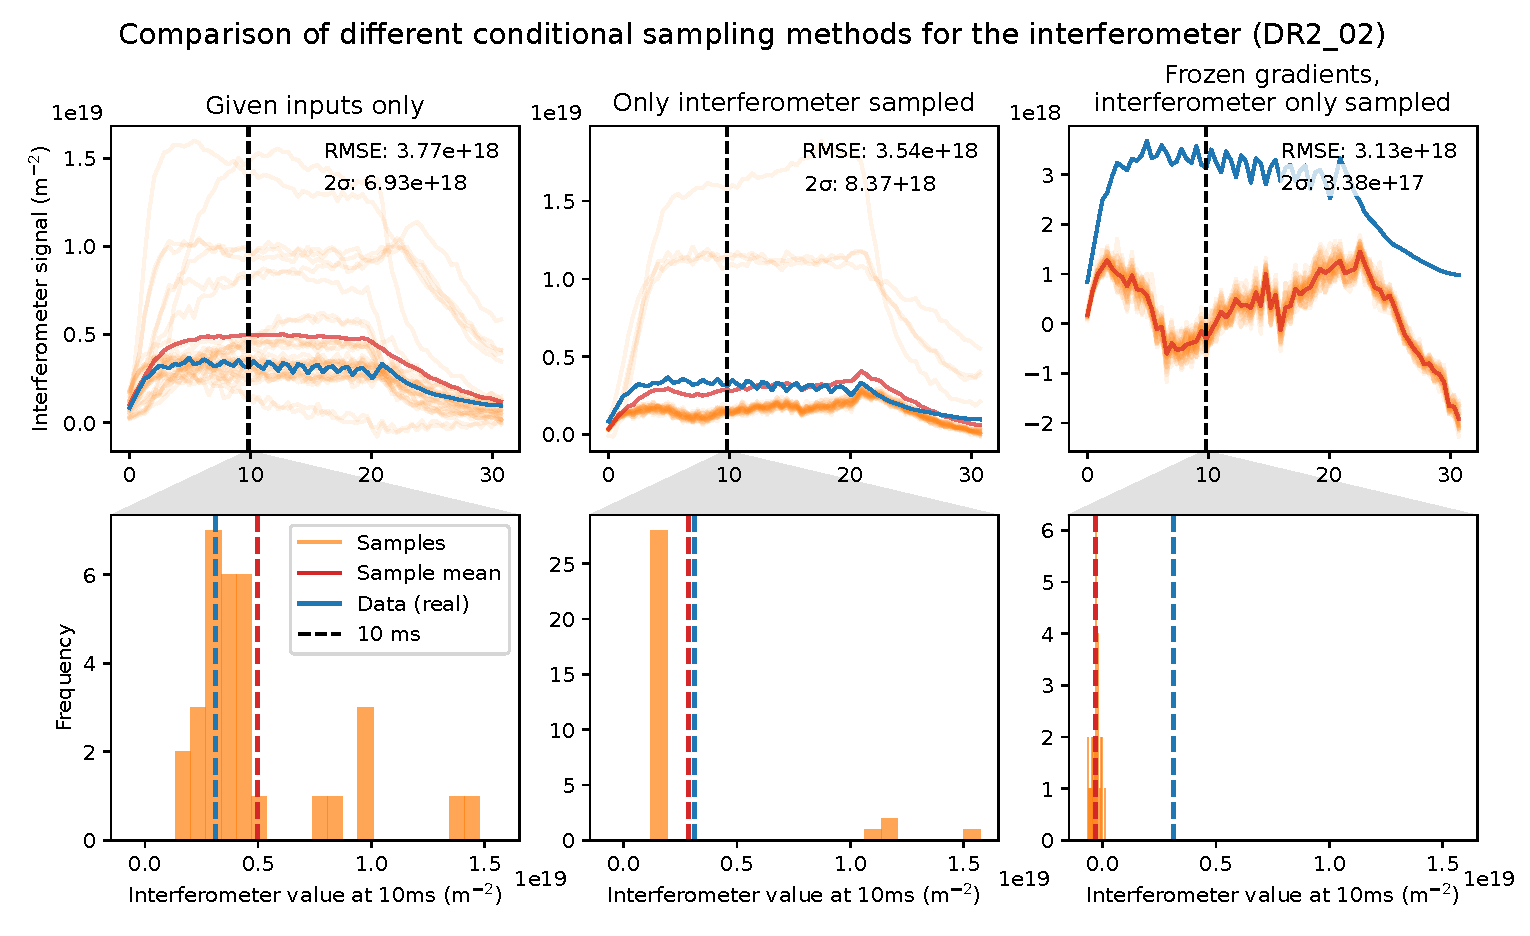
\includegraphics[width=\linewidth]{figures/interferometer_sampling_comp_39-0.pdf}
	\caption{\label{fig:ifo_sample}Reconstructing the interferometer signal for a test-set datarun, showing only 32 samples for clarity. Given only the inputs (left), the interferometer signal reconstruction uncertainty is quite large with many possible modes. When given other diagnostics signals, the RMSE improves by $2 \times 10^{17}$ m$^{-2}$, but the uncertainty increases. If the model is sampled by instead initializing all inputs on real data and freezing the gradients (right), the model produces unphysical results and is poorly calibrated. The datarun chosen (DR2\_02) is representative of performance across the test set. }
\end{figure}

Note that there is nothing special about sampling the interferometer in particular. Any diagnostic or feature of the dataset can be conditionally sampled given other data. In other words, this model allows you to predict any feature of the data given any other feature, which is incredibly powerful, and may enable opportunities such as diagnostic calibration after-the-fact.

\section{Symmetries and trends in the energy function}

Structure in the energy function itself can also be examined to extract insights from the data. One example of this can be seen in scans along the energy function for the x-axis probe position. Since LAPD plasmas are approximately azimuthally symmetric (because of the cylindrical geometry), we expect the energy function to exhibit similar behavior. Given a certain $I_\text{sat}$ time series, we expect the position of the probe to be equally likely if the azimuthal symmetry is perfect. Energy scans along the x axis for a given shot (and $I\text{sat}$ time series) for a training and a test set datarun can be seen in fig. \ref{fig:energy_x_scan}. When a shot near or on the magnetic axis is provided, the energy function is largely symmetric about that point. When a shot is provided further out, the energy function takes on a shape with two minima, indicating that two positions of the energy surface are likely. This behavior is obvious in the test set case of \texttt{DR2\_19} (yellow curve) -- either side of the y axis on the x axis are nearly equally likely. For a shot near the machine wall (red curve), the energy distribution has two minima, but the minimum on the opposite side is closer than ideal, but the true symmetrical position is beyond the limits of the training data. Not all shots yield symmetric energy functions, as seen in the red curve of the training set (left side of fig. \ref{fig:energy_x_scan}). 

\begin{figure}
	\centering
	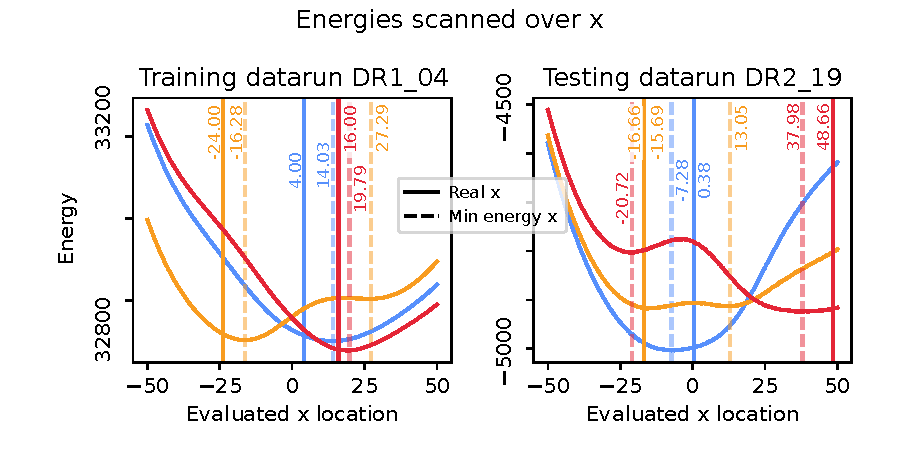
\includegraphics[width=400pt]{figures/energy_x_scan_train-test_39-0}
	\caption{\label{fig:energy_x_scan}Scans along the x-axis input for the energy function of a real shot. When off-axis shots are provided, the energy function may encode the symmetry about the y axis.}
\end{figure}

Certainly other symmetries in the data could be uncovered by directly analyzing this energy function (future work includes the relationship of gas puff duration and voltage to discharge power). Although obvious in retrospect, this energy function symmetry  indicates an important feature of inverse modeling using EBMs. This feature is that if the inversion is not well posed, or has many possible solutions, the EBM will predict many of them and not just the mean. In other words: using the energy function, anything can be predicted from anything else regardless of the invertibility of the problem.

%\section{Improving model using 30 million-shot dataset}

\section{Conclusion}

In this work, we demonstrate using the usefulness of energy-based models (EBMs) for modeling the data distribution. Using a multi-branch, medium-term fusion architecture, signals from multiple time-series diagnostics, machine state information, and LAPD inputs are mapped onto an energy surface. This dataset is highly multimodal in both definitions of the term: the distribution has many modes and the inputs are different modalities. This energy surface is related to a probability distribution via $p(x) = \exp(-E(x))$ and can be easily sampled using Langevin dynamics. The distribution captures all modes of the data, though the represented probability mass has some room for improvement. Using this learned distribution, it is possible to detect anomalies, reconstruct diagnostic signals given other data, and uncover trends or symmetries. When reconstructing diagnostics, additional data is very beneficial, even when the signals are from an uncalibrated diagnostic and are unanalyzed. This result implies that collecting many different diagnostics signals -- even if they are basic -- can be very useful and contain exploitable information. In other words, this model can exploit information we humans cannot, either because of lack of time, manpower, or the complexity of analysis.

This energy-based distributions are amenable to outside modification, as demonstrated by the novel conditional sampling technique in this work. This direct access to the distribution representations enables the scientist the shape the sampling process however desired, so that trends along any input or combination of inputs cam be performed.

\section{Future work}
Given the flexibility of EBMs, there are many potential ways of improving on this work. The most obvious improvement would be to collect additional data from random LAPD configurations. Expanded probe positions would also be useful. This EBM can be extended to include arbitrary amounts of diagnostics, enabling after-the-fact diagnostic calibration or inference of plasma parameters. 

The compositional capabilities of EBMs could enable the model to expand to various machine states (e.g., cathode condition, heater temperature). An EBM could be trained on a 29 million shot dataset which covers various machine states over 3 years. Composing this model with the trained model in this work could enable this model to apply in a broader range of scenarios.

EBMs may also provide a way of joining theory and experiment. One could train an EBM on a diverse array of simulations with a variety of included physics or strengths of various effects. Jointly sampling from the sum of the theory and experiment models will effectively select the appropriate physics model for the desired scenario, enabling better predictive performance of the simulations. 

In summary, EBMs provide a powerful new way of representing and analyzing data from a plasma device, and may become more useful and easier to train as compute becomes cheaper. These EBMs may enable the future automation of fusion science and device optimization.



%The energy surface gradients in MCMC could be broken down on a per-input basis so that each input has its own step size. Adaptive step sizes could also be used. 
%Despite scaling the step size to the lowest standard deviation, the distribution of inputs are multimodal, so the standard deviation along one input may be much greater than the standard deviations of the modes in that input. For example, the flags (off or on) have a standard deviation of zero for each mode, but have a nonzero standard deviation when scaled according to the mean and peak-to-peak values. Data augmentation may be useful here to artificially spread the size of these delta-function inputs.
%
%High-dimensional, multimodal inputs on EBMs have been relatively unexplored. Multimodal inputs introduce new challenges to the sampler. The importance of each input on the gradient is no long identical -- some parameters are more important (e.g., field strength) than, say, a single time step of the diode signal. 
%
%This work could be extended with more randomly-sampled data from the Large Plasma Device
%
%Curriculum learning could be an interesting way to improve model stability and distribution similarity (between the training data and sampled data).
%
%This model can be composed with another EBM trained on an auxiliary dataset toz improve model performance across different LAPD modes of operation.